\documentclass[10pt]{article}
\usepackage[utf8]{inputenc}
\usepackage[T1]{fontenc}
\usepackage{amsmath}
\usepackage{amsfonts}
\usepackage{amssymb}
\usepackage{mhchem}
\usepackage{stmaryrd}
\usepackage{bbold}
\usepackage{graphicx}
\usepackage[export]{adjustbox}
\graphicspath{ {./images/} }

\title{Ph.D. Qualifying Exam and M.S. Comprehensive Exam in Algebra }


\author{Professors Frauke Bleher and Miodrag Iovanov}
\date{}


\begin{document}
\maketitle

Aug 18, 2020, 1.00 - 4:00 p.m. in S207 PBB

\section*{Instructions: }
\begin{itemize}
  \item Do exactly two problems from each of the four sections.

  \item Justify your answers and show your work.

  \item Please write legibly.

  \item In answering any part of a question, you may assume the results in previous parts, even if you have not solved them.

  \item Unless specified otherwise, each problem is worth 15 points with points equidistributed across all parts within a given problem.

\end{itemize}
Notations: We adopt standard notations. Namely, we write $\mathbb{C}, \mathbb{R}$ and $\mathbb{Q}$ to denote the field of complex numbers, real numbers and rational numbers, respectively; we write $\mathbb{Z}$ to denote the ring of rational integers. Throughout this exam, $R$ denotes a ring with identity $1 \neq 0 ; R$ is called an integral domain if it is commutative with no zero divisors. All $R$ modules are assumed to be unital left modules. For any set $X$, we write $|X|$ to denote its cardinality.

\section{Groups}
\begin{enumerate}
  \item Suppose $G$ is a group such that $|G|=2 k$ with $k$ odd. Prove that $G$ has a subgroup of order $k$.

  \item Let $p$ be a prime number and let $\mathbb{F}_{p}$ denote the finite field with $p$ elements. Consider the group $G=G L_{2}\left(\mathbb{F}_{p}\right)$ consisting of all $2 \times 2$ invertible matrices with entries in $\mathbb{F}_{p}$.

\end{enumerate}
(i) Determine the order of the group $G$.

(ii) Exihibit a Sylow $p$-subgroup of $G$.

(iii) Determine the number of Sylow $p$-subgroups of $G$.

\begin{enumerate}
  \setcounter{enumi}{3}
  \item Prove that a finite simple group of even order can be generated by a set of elements of order 2. (A group $G$ is said to be simple if it is non-trivial and has no normal subgroups besides $\{e\}$ and $G$ itself.)
\end{enumerate}
\section{Rings}
\begin{enumerate}
  \item Let $R$ be a commutative ring with 1. It is said to be Noetherian if it satisfies the ascending chain condition on ideals:
\end{enumerate}
(i) If $\mathfrak{a}_{1} \subseteq \mathfrak{a}_{2} \subseteq \cdots \subseteq \mathfrak{a}_{k} \subseteq \cdots$ is an ascending chain of ideals in $R$, then $\mathfrak{a}_{k}=$ $\mathfrak{a}_{k+1}=\cdots$ for a sufficiently large $k$.

Alternately, if the following is satisfied:

(ii) Every ideal of $R$ is finitely generated.

Show that (i) $\Longleftrightarrow$ (ii).

\begin{enumerate}
  \setcounter{enumi}{2}
  \item An arithmetic function is a complex valued function on the set of positive integers $\mathbb{Z}^{+}=\{1,2,3, \ldots\}$. Let $\mathcal{A}$ be the set of all arithmetic functions. Define the sum in $\mathcal{A}$ to be the ordinary addition of functions, and define a product $\star$ by the formula
\end{enumerate}
$$
f \star g(m)=\sum_{x y=m} f(x) g(y)
$$
(a) (5 points) Show that $\mathcal{A}$ is a commutative ring whose unit element is the function $\delta$ such that $\delta(1)=1$ and $\delta(x)=0$ if $x \neq 1$.

(b) (10 points) Show that an element $f \in \mathcal{A}$ is invertible if and only if $f(1) \neq 0$. 3. Consider the Gaussian ring $\mathbb{Z}[i]$ and the natural homomorphism
$$
\phi: \mathbb{Z} \rightarrow \mathbb{Z}[i] /(6+i)
$$
given by $a \mapsto a+(6+i)$.\\
(a) ( 7 points) Show that $\phi$ is surjective.\\
(b) (8 points) Prove that $\mathbb{Z}[i] /(6+i) \cong \mathbb{Z}_{37}$.

\section{Linear Algebra and Module Theory}
\begin{enumerate}
  \item Let $F$ be a field and consider the vector space $V$ given by
\end{enumerate}
$$
V=F[x] /(x+1)^{2} \oplus F[x] /\left(x^{2}-1\right) \oplus F[x] /(x-1)^{2}
$$
as a direct sum of cyclic $F[x]$-modules.

(a) (8 points) Determine the invariant factors and elementary divisors of $V$ as a $F[x]$-module.

(b) ( 7 points) Determine the rational canonical form of the linear transformation $T: V \longrightarrow V$ given by multiplication by $x .$

\begin{enumerate}
  \setcounter{enumi}{2}
  \item Let $V$ be the vector space over $\mathbb{R}$ of real polynomials whose degree $\leq n$. Let $T$ : $V \longrightarrow V$ be the linear map given by
\end{enumerate}
$$
T(p(x))=p^{\prime}(x)
$$
Determine the Jordan canonical form and the rational canonical form of $T$.

\begin{enumerate}
  \setcounter{enumi}{3}
  \item Let $R$ be a commutative ring, let $M$ and $N$ be $R$-modules, and $\operatorname{Hom}_{R}(M, N)$ denote the set of $R$-module homomorphisms $M \rightarrow N$.
\end{enumerate}
(a) (5 points) Describe the natural $R$-module structure on $\operatorname{Hom}_{R}(M, N)$ with a short justification.

(b) (10 points) Now let $R=\mathbb{Z}$ and $M=\mathbb{Z} /(m)$ and $N=\mathbb{Z} /(n)$, where $m, n$ are positive integers. Describe $\operatorname{Hom}_{\mathbb{Z}}(M, N)$ as a direct sum of cyclic $\mathbb{Z}$-modules, including a complete proof that your description is correct.

\section{Field Theory}
\begin{enumerate}
  \item Suppose $f(x) \in \mathbb{Q}[x]$ is a monic polynomial of degree $n$ and $\alpha_{1}, \alpha_{2}, \ldots, \alpha_{n} \in \mathbb{C}$ are the roots of $f(x)$. Let $G$ be the Galois group of $f$ over $\mathbb{Q}$.
\end{enumerate}
(a) (9 points) Show that $f(x)$ is irreducible in $\mathbb{Q}[x]$ if and only if the action of $G$ on $\left\{\alpha_{1}, \alpha_{2}, \ldots, \alpha_{n}\right\}$ is transitive.

(b) $(6$ points ) If $f(x)$ is irreducible in $\mathbb{Q}[x]$, then show that $n$ divides $|G|$.

\begin{enumerate}
  \setcounter{enumi}{2}
  \item Let $K$ be the splitting field of $f(x)=x^{4}-4 x^{2}+2$ over $\mathbb{Q}$.
\end{enumerate}
(a) (9 points) Determine the Galois group of $K$ over $\mathbb{Q}$.

(b) (6 points) Find all quadratic subfields of $K$.

\begin{enumerate}
  \setcounter{enumi}{3}
  \item Let $E / F$ be a finite extension of fields.
\end{enumerate}
(a) Give a detailed definition for the property that $\underline{E}$ is Galois over $F$.

Note that different textbooks may use different definitions. Any definition which is equivalent to the standard one in Dummit and Foote (in the finite case) is acceptable here, but you must include additional definitions for any terminology from field theory that you use in your definition.

(b) Let $\alpha=\sqrt[4]{2} \in \mathbb{R}$ be the real fourth root of 2 . Using the definition you provided in part (a), demonstrate whether $\mathbb{Q}[\alpha]$ is Galois over $\mathbb{Q}$ or not.

(c) Let $F$ be a field of characteristic not equal to 2 , and suppose $E / F$ is degree 2 . Use the definition you provided in (a) to prove that $E$ is Galois over $F$.

(d) Give an example of a tower of Galois extensions that is not Galois, meaning, a tower of fields $F \subset E \subset K$ so that $E$ is Galois over $F, K$ is Galois over $E$, but $K / F$ is not Galois.

\section*{Ph.D. Qualifying Exam and M.S. Comprehensive Exam in Algebra }

January 17, 2020

\section*{Instructions: }
\begin{itemize}
  \item Do EXACTLY TWO problems from EACH of the four sections.

  \item Please start a new page for every new problem and put your name on each sheet.

  \item Justify your answers and show your work.

  \item Please write legibly.

  \item In answering any part of a question, you may assume the results in previous parts of the SAME question, even if you have not solved them.

  \item Please turn in the exam questions with your solutions.

\end{itemize}
\section{Notations:}
We adopt standard notations. Namely:

\begin{itemize}
  \item We write $\mathbb{C}, \mathbb{R}$ and $\mathbb{Q}$ to denote the field of complex numbers, real numbers and rational numbers, respectively. We write $\mathbb{Z}$ to denote the ring of rational integers. If $p$ is a prime number and $q=p^{k}(k \geq 1)$, then $\mathbb{F}_{q}$ denotes the finite field with $q$ elements.

  \item Throughout this exam, $R$ denotes a ring with identity $1 \neq 0 ; R$ is called an integral domain if it is commutative with no zero divisors.

  \item All $R$-modules are assumed to be unital left $R$-modules.

\end{itemize}
\section{Groups}
\begin{enumerate}
  \item Let $G$ be a finite $p$-group, with $p \geq 2$ a prime number.
\end{enumerate}
(i) Prove that $Z(G)$ is non-trivial.

(ii) If $G / Z(G)$ is cyclic, prove that $G$ is abelian.

(iii) Show that if $|G|=p^{2}$, then $G$ is isomorphic to either $\mathbb{Z}_{p^{2}}$ or $\mathbb{Z}_{p} \times \mathbb{Z}_{p}$.

\begin{enumerate}
  \setcounter{enumi}{2}
  \item Prove that a finite simple group of even order can be generated by a set of elements of order 2 .

  \item Let $p<q$ be prime integers.

\end{enumerate}
(i) Show that if $p$ does not divide $q-1$, then any group of order $p q$ is cyclic.

(ii) Give an example of a non-cyclic group of order $p q$ when $p$ does divide $q-1$.

\section{Rings}
\begin{enumerate}
  \item Show that there is an isomorphism of rings
\end{enumerate}
$$
\frac{\mathbb{Z}[X]}{\left\langle 2, X^{3}+X+1\right\rangle} \cong \frac{\mathbb{Z}[X]}{\left\langle 2, X^{3}+X^{2}+1\right\rangle}
$$

\begin{enumerate}
  \setcounter{enumi}{2}
  \item Let $R$ be a commutative ring with 1. Call ideals $I, J$ relatively prime if $I+J=R$. Prove the following two statements independently (i.e., statement (i) is not used to prove statement (ii)).
\end{enumerate}
(i) Assume $I, J$ are relatively prime and $I \cap J=0$. Prove that $R \cong R / I \times R / J$.

(ii) Prove that if $I$ and $J$ are relatively prime, so are $I^{m}$ and $J^{n}$ for any positive integers $m, n$.

\begin{enumerate}
  \setcounter{enumi}{3}
  \item Let $R$ be a commutative ring with 1 and $a \in R$. Prove the following two statements independently (i.e., statement (i) is not used to prove statement (ii)).
\end{enumerate}
(i) If $P \subset R$ is a prime ideal such that $P \subsetneq(a)$, prove that $P=a P$.

(ii) Suppose that $(a)$ is a maximal ideal of $R$. Prove that there is no ideal $I$ of $R$ satisfying $(a) \supsetneq I \supsetneq\left(a^{2}\right)$.

\section{Linear Algebra and Module Theory}
\begin{enumerate}
  \item Let $S, T: \mathbb{C}^{n} \rightarrow \mathbb{C}^{n}$ be linear operators such that $S T=T S$. Prove that $S$ and $T$ have a common eigenvector.

  \item Let $d \geq 1$ be an integer and $V \subset \mathbb{C}[x]$ the complex vector space of polynomials of degree $\leq d$. Consider the linear transformation $T: V \rightarrow V$ sending a polynomial $P(x)$ to $P(x-1)$.

\end{enumerate}
(i) Find all eigenvectors and eigenvalues of $T$.

(ii) Use part (i) to find the Jordan canonical form of $T$.

\begin{enumerate}
  \setcounter{enumi}{3}
  \item Let $A$ be a $\mathbb{Z}$-module, $n$ a positive integer, and define
\end{enumerate}
$$
A_{n}=\{a \in A \mid n a=0\}
$$
which you may assume is a $\mathbb{Z}$-module without proof. Construct (with proof) an isomorphism of $\mathbb{Z}$-modules $\operatorname{Hom}_{\mathbb{Z}}(\mathbb{Z} / n \mathbb{Z}, A) \cong A_{n}$.

\section{Field Theory}
\begin{enumerate}
  \item Let $p$ be a prime integer and $\alpha$ a root of the polynomial $x^{3}-p$.
\end{enumerate}
(i) Find (with justification) the degree of the field extension $\mathbb{Q}(\alpha, i)$ over $\mathbb{Q}$, where $i=\sqrt{-1}$ as usual.

(ii) Prove that $x^{3}-p$ is irreducible in the polynomial ring $\mathbb{Q}(i)[x]$.

\begin{enumerate}
  \setcounter{enumi}{2}
  \item Determine (with proof) the Galois group $G$ of the splitting field $F$ of the polynomial $x^{20}-1$ over $\mathbb{Q}$. Use this to describe to describe all intermediate fields between $\mathbb{Q}$ and $F$, along with their degrees, and which are normal extensions of $\mathbb{Q}$.

  \item Give an explicit description of all intermediate fields between $\mathbb{Q}$ and $\mathbb{Q}(\sqrt[3]{5}, \zeta)$, where $\zeta$ is a primitive $3 \mathrm{rd}$ root of $1 .$

\end{enumerate}
\section*{Ph.D. Qualifying Exam and M.S. Comprehensive Exam in Algebra }

August 18, 2017, 9:00 a.m. - 12:00 p.m. in $221 \mathrm{MLH}$

\section*{Instructions: }
\begin{itemize}
  \item Do EXACTLY TWO problems from EACH of the four sections.

  \item Please start a new page for every new problem and put your name on each sheet.

  \item Justify your answers and show your work.

  \item Please write legibly.

  \item In answering any part of a question, you may assume the results in previous parts of the SAME question, even if you have not solved them.

  \item Please turn in the exam questions with your solutions.

\end{itemize}
\section{Notations:}
We adopt standard notations. Namely:

\begin{itemize}
  \item We write $\mathbb{C}, \mathbb{R}$ and $\mathbb{Q}$ to denote the field of complex numbers, real numbers and rational numbers, respectively; we write $\mathbb{Z}$ to denote the ring of rational integers.

  \item Throughout this exam, $R$ denotes a ring with identity $1 \neq 0 ; R$ is called an integral domain if it is commutative with no zero divisors.

  \item All $R$-modules are assumed to be unital left $R$-modules.

\end{itemize}
\section{Groups}
\begin{enumerate}
  \item Let $G$ be a group that acts transitively on a finite set $A$. ( $G$ is NOT assumed to be finite.) Let $H$ be a normal subgroup of $G$, and let $\mathcal{O}_{1}, \ldots, \mathcal{O}_{r}$ be the distinct orbits of $H$ on $A$.
\end{enumerate}
Prove that the action of $G$ on $A$ induces a well-defined action of $G$ on $\left\{\mathcal{O}_{1}, \ldots, \mathcal{O}_{r}\right\}$, and prove that this action is transitive. Deduce that all orbits of $H$ on $A$ have the same cardinality.

\begin{enumerate}
  \setcounter{enumi}{2}
  \item Let $p$ be a prime number. If $G$ is a finite group, denote the number of Sylow $p$ subgroups of $G$ by $n_{p}(G)$. Suppose $A$ and $B$ are finite groups, and that $P$ is a Sylow $p$-subgroup of $A$ and $Q$ is a Sylow $p$-subgroup of $B$.
\end{enumerate}
Prove that $P \times Q$ is a Sylow $p$-subgroup of $A \times B$, and that $n_{p}(A \times B)=n_{p}(A) n_{p}(B)$.

\begin{enumerate}
  \setcounter{enumi}{3}
  \item Let $G$ be a group with identity element $e$. Suppose $n>1$ is a fixed integer such that $(x y)^{n}=x^{n} y^{n}$ for all $x, y \in G$. Define
\end{enumerate}
$$
G^{(n)}=\left\{x^{n} \mid x \in G\right\} \quad \text { and } \quad G_{(n)}=\left\{x \in G \mid x^{n}=e\right\} .
$$
(a) Show that $G^{(n)}$ and $G_{(n)}$ are normal subgroups of $G$.

(b) If $G$ is finite, show that the order of $G^{(n)}$ equals the index of $G_{(n)}$ in $G$.

(c) Show that for all $x, y \in G$, we have $x^{1-n} y^{1-n}=(x y)^{1-n}$. Use this to deduce that $x^{n-1} y^{n}=y^{n} x^{n-1}$.

\section{Rings}
\begin{enumerate}
  \item Let $n \geq 2$ be an integer, and $\operatorname{let}_{\operatorname{Mat}}^{n}$ entries in $R$.
\end{enumerate}
Prove that every two-sided ideal of $\operatorname{Mat}_{n}(R)$ is equal to $\operatorname{Mat}_{n}(J)$ for some two-sided ideal $J$ of $R$.

\begin{enumerate}
  \setcounter{enumi}{2}
  \item Let $R$ be an integral domain.
\end{enumerate}
(a) Prove that every prime element in $R$ is irreducible in $R$. (Please include definitions of irreducible and prime elements.)

(b) If $R$ is a Principal Ideal Domain, prove that the converse is also correct.

\begin{enumerate}
  \setcounter{enumi}{3}
  \item Determine which of the following ideals are prime ideals. Please justify your answers.\\
(a) The ideal generated by $i$ in the ring of Gaussian integers $\mathbb{Z}[i]$.\\
(b) The ideal generated by $y$ and $x^{2}+y x+1$ in $\mathbb{Z}[x, y]$.\\
(c) The ideal generated by $y^{2}-x^{3}-x^{2}$ in $\mathbb{C}[x, y]$.
\end{enumerate}
\section{Linear Algebra and Module Theory}
\begin{enumerate}
  \item Suppose
\end{enumerate}
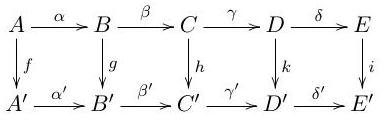
\includegraphics{2022_05_24_f62df93b9d660067b55fg-10}

is a commutative diagram of $R$-modules with exact rows.

Prove: If $g$ and $k$ are isomorphisms, $f$ is surjective and $i$ is injective, then $h$ is an isomorphism.

\begin{enumerate}
  \setcounter{enumi}{2}
  \item Let $F$ be a field and let $V$ be a vector space over $F$. Let $V^{*}=\mathrm{Hom}_{F}(V, F)$ be the dual vector space of $V$ and let $V^{* *}=\left(V^{*}\right)^{*}$ be its double dual. Define a map $\tau: V \rightarrow V^{* *}$ by $\tau(v)(f)=f(v)$ for all $v \in V$ and $f \in V^{*}$.\\
(a) Prove that $\tau$ is an injective linear transformation.\\
(b) If $V$ is finite dimensional over $F$, prove that $\tau$ is an isomorphism.

  \item A module over a ring $R$ is simple if it has no non-zero proper submodules and it is semi-simple if it is a direct sum of simple modules. One defines a linear operator $T$ on a finite dimensional vector space $V$ (over a field $k$ ) to be semi-simple if the corresponding $k[x]$-module $(V, T)$ is semi-simple.\\
(a) Describe all simple $k[x]$-modules. Please justify your answer.\\
(b) Show that if $T$ is diagonalizable, then it is semi-simple. Show that the converse holds if $k$ is algebraically closed.

\end{enumerate}
\section{Field Theory}
\begin{enumerate}
  \item Let $p$ be a prime number, let $f(x)=x^{p}-5 \in \mathbb{Q}[x]$, and let $G$ be the Galois group of the splitting field of $f(x)$ over $\mathbb{Q}$.
\end{enumerate}
Prove that $G$ is isomorphic to the group of matrices
$$
\left\{\left(\begin{array}{ll}
a & b \\
0 & 1
\end{array}\right) \mid a, b \in \mathbb{F}_{p}, a \neq 0\right\} .
$$

\begin{enumerate}
  \setcounter{enumi}{2}
  \item Let $F \subseteq K \subseteq L$ be a tower of fields.
\end{enumerate}
Prove: $L / F$ is an algebraic extension if and only if $L / K$ and $K / F$ are both algebraic extensions.

\begin{enumerate}
  \setcounter{enumi}{3}
  \item Determine the order of the Galois group of $K / \mathbb{Q}$ where $K$ is the splitting field of $f(x)=x^{6}-4 x^{3}+1$ over $\mathbb{Q} .$ PH.D. QUALIFYING EXAM IN AlGEBRA
\end{enumerate}
Friday, January 13, 2006

Professors Frauke Bleher and Fred Goodman

Instructions: This exam has 4 parts. Do exactly 2 problems from each of the 4 parts. Responses will be judged for correctness, completeness, clarity and orderliness. Justify all statements.

\begin{enumerate}
  \item GrouPS:
\end{enumerate}
(1) Let $Z$ be the center of a group $G$, and suppose that $G / Z$ is cyclic. Prove that $G$ is abelian.

(2) Let $A$ be a finite abelian group, written additively, with $|A|=n \geq 2$. For $m \in \mathrm{Z}^{+}$, define $A_{m}=\{x \in A \mid m x=0\}$. If $n=m \cdot m^{\prime}$, where $m, m^{\prime} \in \mathbb{Z}^{+}$ and $\operatorname{gcd}\left(m, m^{\prime}\right)=1$, show that $A=A_{m} \oplus A_{m^{\prime}}$. Please do not cite a heorem, but prove this from scratch.

(3) In this exercise you may wish/need to use that the automorphism group of $\mathbb{Z}_{7}$ is isomorphic to $\mathbb{Z}_{6}$

(a) Show that any group $G$ of order 28 has a normal subgroup $N$ of order 7. Let $A$ denote a 2-Sylow subgroup, of order 4 . Show that $G$ is the semi-direct product of $N$ and $A$.

(b) Show that there exists a non-abelian group of order 28 with 2-Sylow subgroup isomorphic to $\mathbb{Z}_{2} \times \mathbb{Z}_{2}$

(c) Show that there exists a non-abelian group of order 28 with 2-Sylow subgroup isomorphic to $Z_{4}$.

(4) (a) Show that for any abelian group, $x \mapsto x^{-1}$ is a group automorphism of order 2. In particular, $\alpha:[x] \mapsto[-x]$ is an automorphism of $\mathbb{Z}_{n}$ of order $2 .$

(b) Show that $\mathbb{Z}_{n} \times \mathbb{Z}_{2}$ is isomorphic to the dihedral group $D_{n}$ of order $2 n$ (defined as the group of symmetries of the regular $n$-gon.)

(c) Determine the center of $D_{n}$. Note that the answer is different for $n$ even and odd.

\begin{enumerate}
  \setcounter{enumi}{2}
  \item RINGS:
\end{enumerate}
All rings are assumed to have a multiplicative identity $1 .$

(1) Let $K$ be a field

(a) Prove that $K[t]$ is a Euclidean domain.

(b) Prove that every Euclidean domain is a principal ideal domain.

(2) Prove that a commutative ring with identity is a field if, and only if, it is simple. (3) Let $R$ be a unique factorization domain, and let $p$ be a prime element in

$\left.R_{(p)}=\{a / b \mid a, b \in R, p)_{1} b\right\} .$

Prove that $R_{(p)}$ is a principal ideal domain. Describe all ideals of $R_{(p)}$ and state which ones are maximal.

(4) Let $R$ be an integral domain, let $J$ be an ideal in $R$, and let $p$ be a nonzero, nonunit element of $R$.

(a) Show that $J$ is maximal ideal $\Longrightarrow J$ is a prime ideal.

(b) Show that $p$ is a prime element $\Longrightarrow p$ is irreducible

(c) If $R$ is a principal ideal domain, show that $p$ is irreducible $\Rightarrow p R$ is

a maximal ideal.

(d) Give an example of an integral domain $R$ and an irreducible element $p$ such that $p R$ is not a maximal ideal.

\begin{enumerate}
  \setcounter{enumi}{3}
  \item FiELDS:
\end{enumerate}
(1) Let $F$ be a field and let $t$ be transcendental over $F$ (i.e. not algebraic). Let $x \in F(t)$ and suppose $x \notin F$. Write $x$ as a quotient of relatively prime polynomials, $x=f(t) / g(t)$. Prove that $F(t)$ is algebraic over $F(x)$ and express the degree $[F(t): F(x)]$ in terms of the degrees of $f(t)$ and $g(t)$.

(2) Let $F$ be a field, and let $f(t) \in F[t]$ be a polynomial of degree $\geq 1$

(a) Give the definition of a splitting field of $f(t)$ over $F$.

(b) Prove that there exists a splitting field of $f(t)$ over $F$.

(3) Let $f(x)=x^{3}-2$. Prove that $f(x)$ is irreducible over $\mathbb{Q}$. Determine the splitting field $K$ of $f(x)$ over $\mathbb{Q}$ and the degree $[K: \mathbb{Q}]$. Write down all the permutations on the roots of $f$ that are induced by elements of $\operatorname{Gal}(K / \mathbb{Q})$ Determine the isomorphism type of $\operatorname{Gal}(K / \mathbb{Q})$.

(4) Let $f(x)$ be an irreducible polynomial of degree $n$ over a field $K$ of characteristic 0 . Define the Galois group of $f(x)$ over $K$. Show that the Galois group of $f(x)$ acts faithfully and transitively on the roots of $f(x)$ in a splitting field. Do not quote any big theorem, such as the fundamental theorem of Galois theory, but prove this from scratch.

\begin{enumerate}
  \setcounter{enumi}{4}
  \item LINEAR ALGEBRA AND MODULES:
\end{enumerate}
(1) Let $V$ be a finite dimensional vector space over a field $K, V \neq\{0\}$. Let $R=\operatorname{End}_{K}(V)$. Define a left $R$-module structure on $V$ by $f v=f(v)$ for all $f \in R$ and all $v \in V$. Prove that this makes $V$ into a left $R$-module, and prove that $V$ is a simple left $R$-module, i.e. the only $R$-submodules of $V$ are $\{0\}$ and $V$ (2) Let $V$ be a finite dimensional vector space over a field $K, V \neq\{0\}$, and let $A, B: V \rightarrow V$ be $K$-linear maps.

(a) Show that the eigenvalues of $A B$ are the same as the eigenvalues of $B A$.

(b) Suppose $A$ is invertible and $\lambda$ is an eigenvalue of $A$. Prove that $\lambda \neq 0$ and that $\lambda^{-1}$ is an eigenvalue of $A^{-1}$

(3) (a) Determine the possible Jordan canonical forms for a nilpotent 4-by-4 matrix.

(b) Show that if $A$ is a nilpotent $n$-by- $n$ matrix, then $E+A$ is invertible, where $E$ is the $n-\mathrm{by}-n$ identity matrix.

(4) Consider the matrix
$$
A=\left[\begin{array}{rrrr}
1 & 2 & -4 & 4 \\
2 & -1 & 4 & -8 \\
1 & 0 & 1 & -2 \\
1 & 1 & -2 & 3
\end{array}\right]
$$
The characteristic polynomial of $A$ is
$$
\chi_{A}(x)=(x-1)^{2}(x+1)(x-3) .
$$
Find the Jordan canonical form over $\mathbb{C}$ of the matrix $A$ and find an invertible matrix $P$ such that $P^{-1} A P$ is the Jordan form of $A$. PH.D. QUALIFYING EXAM AND M.S. COMPREHENSIVE EXAM IN ALGEBRA

Wednesday, January 23, 2008

Professors Frauke Bleher and Vic Camillo

Instructions: Do exactly two problems from each section for a total of eight problems. Be sure to justify your answers. Good luck.

\begin{enumerate}
  \item GROUPS:
\end{enumerate}
(1) Let $G$ be a group of order 30 . Show that $G$ has a normal subgroup of order 15. You may use the Sylow Theorems.

(2) Let $G$ be a finite group. Show that the order of any subgroup of $G$ divides the order of $G$. Do not quote any theorems, but prove this from scratch.

(3) Suppose $T$ and $H$ are groups and that $\varphi, \varphi^{\prime}: T \rightarrow \operatorname{Aut}(H)$ are homomorphisms. Suppose there is an isomorphism $\alpha: T \rightarrow T$ such that
$$
\varphi^{\prime} \circ \alpha=\varphi \text {. }
$$
Show that the semi-direct products $H \rtimes_{\varphi} T$ and $H \rtimes_{\varphi^{\prime}} T$ are isomorphic. (Here $H$ is the normal subgroup in these semi-direct products.)

Hint: Use $\alpha$ to define a set map from the product set $H \times T$ to itself.

(4) Let $G$ be a group (finite or infinite). Prove that if $H$ is a subgroup of finite index $n$, then $G$ contains a normal subgroup $K$ with $K \leq H$ and $|G: K| \leq n$ ! .

Hint: Use the natural action of $G$ on the left cosets of $H$ in $G$.

\section{RINGS:}
All rings are assumed to have a multiplicative identity 1 .

(1) An element in a ring $R$ is called irreducible, if whenever $p=x y$, where $x$ and $y$ are elements of $R$, then one of $x$ or $y$ is a unit. Let $R$ be principal ideal domain and $p$ an irreducible element in $R$. Show directly that if $p$ divides $a b$, where $a$ and $b$ are elements of $R$, then $p$ divides $a$ or $p$ divides $b$.

(2) Let $R$ be a commutative ring. Recall that an ideal $M$ in $R$ is called maximal if $M$ is not equal to $R$ and if $I$ is an ideal in $R$ with $M \subseteq I \subseteq R$ then $M=R$ or $M=I$. Show that $M$ is a maximal ideal of $R$ if and only if $R / M$ is a field.

(3) Let $R$ be a ring. Recall that an element $x \in R$ is called nilpotent if $x^{n}=0$ for some $n \in \mathbb{Z}^{+}$.

(a) Suppose $R$ is commutative. Prove that the set
$$
N(R)=\{x \in R \mid x \text { nilpotent }\}
$$
is an ideal in $R$. This is called the nilradical of $R$. (b) Prove that the elements $x=\left(\begin{array}{ll}0 & 1 \\ 0 & 0\end{array}\right)$ and $y=\left(\begin{array}{cc}0 & 0 \\ 1 & 0\end{array}\right)$ are nilpotent elements in the matrix ring $\operatorname{Mat}_{2}(\mathbb{Z})$. Prove that $x+y$ is not nilpotent, and deduce that the set of nilpotent elements in $\operatorname{Mat}_{2}(\mathbb{Z})$ is not an ideal.

(4) Show directly the following variant of Eisenstein's criterion: Let $P$ be a prime ideal in the unique factorization domain $R$ and let $f(x)=a_{n} x^{n}+$ $\cdots+a_{1} x+a_{0}$ be a polynomial in $R[x]$ where $n \geq 1$. Suppose $a_{n} \notin P$ $a_{n-1}, \ldots, a_{0} \in P$ and $a_{0} \notin P^{2}$. Prove that $f(x)$ is irreducible in $F[x]$, where $F$ is the fraction field of $R$.

\section{FIELDS:}
(1) Let $F$ be a field and let $g(x)$ be an irreducible polynomial over $F$. Show directly that there is an extension field of $F$ in which $g(x)$ has a root.

(2) Let $f(x)=x^{3}+2 x^{2}+2 x+1 \in \mathbb{Q}[x]$. Determine the Galois group of $f(x)$ over $\mathbb{Q}$. Please show all your work.

(3) Let $F$ be a field of characteristic 0 , and let $E / F$ be finite field extension of degree $n$. Let $A$ be an algebraically closed field containing $F$. Let $\sigma_{1}, \ldots, \sigma_{n}$ be all the distinct embeddings of $E$ over $F$ into $A$ (i.e. $\sigma_{i}$ extends the identity on $F$ for all $1 \leq i \leq n$ ). For $\alpha \in E$, define the trace and norm of $\alpha$, respectively, from $E$ to $F$ by
$$
\begin{aligned}
\operatorname{Tr}_{F}^{E}(\alpha) &=\sum_{i=1}^{n} \sigma_{i} \alpha=\sigma_{1} \alpha+\cdots+\sigma_{n} \alpha \\
\mathrm{N}_{F}^{E}(\alpha) &=\prod_{i=1}^{n} \sigma_{i} \alpha=\sigma_{1} \alpha \cdots \sigma_{n} \alpha
\end{aligned}
$$
(a) If $\alpha$ is algebraic over $F$, let
$$
p(t)=\operatorname{Irr}(\alpha, F, t)=t^{n}+a_{n-1} t^{n-1}+\cdots+a_{0} .
$$
Show that $\operatorname{Tr}_{F}^{F(\alpha)}(\alpha)=-a_{n-1}$ and $\mathrm{N}_{F}^{F(\alpha)}(\alpha)=(-1)^{n} a_{0}$.

(b) Let $E / F$ be a finite extension with $[E: F]=n$, and let $a \in F$. Determine $\operatorname{Tr}_{F}^{E}(a)$ and $\mathrm{N}_{F}^{E}(a)$.

(4) Let $F$ be a field of characteristic 0 and let $n \in \mathbb{Z}^{+}$. Let $\zeta$ be a primitive $n$-th root of unity in some extension field of $F$, and let $K=F(\zeta)$. Prove that $K$ is Galois and abelian over $F$.

\section{LINEAR ALGEBRA AND MODULES:}
All rings are assumed to have a multiplicative identity 1 . If $M$ is a left $R$-module, we assume that $1 m=m$ for all $m \in M$.

(1) Let $R$ be an integral domain and let $M$ be a module over $R$. Define $\operatorname{Tor}(M)=\{m \in M \mid a m=0$ for some nonzero element $a \in R\}$. Show that $\operatorname{Tor}(M)$ is a submodule of $M$. (2) Let $R$ be a ring, let $M$ be a right $R$-module, and let $A$ be a right ideal in $R$. Define
$$
X=\left\{\sum m_{k} a_{k} \mid m_{k} \in M \text { and } a_{k} \in A\right\} .
$$
Here, the sums are finite but may have a different number of non zero terms. Show that $X$ is a submodule of $M$.

(3) Let $R$ be a ring with 1 and let $A_{1}$ and $A_{2}$ be left $R$-modules. Suppose $B_{1} \subset A_{1}$ and $B_{2} \subset A_{2}$ are submodules. Prove that
$$
\left(A_{1} \oplus A_{2}\right) /\left(B_{1} \oplus B_{2}\right) \cong\left(A_{1} / B_{1}\right) \oplus\left(A_{2} / B_{2}\right)
$$
as $R$-modules.

(4) Determine the Jordan normal form over $\mathbb{C}$ for the matrix
$$
\left[\begin{array}{rrrr}
0 & 0 & -1 & 2 \\
2 & -2 & -1 & 2 \\
0 & 0 & -2 & 0 \\
0 & 0 & 1 & -2
\end{array}\right]
$$
and determine a matrix $P$ which conjugates this matrix into its Jordan normal form. PH.D. QuALIFYING EXAM AND M.S. COMPREHENSIVE EXAM IN AlGeBRA

Wednesday, August 17, 2005

Professors Frauke Bleher and Fred Goodman

Instructions: This exam has 4 parts. Do exactly 2 problems from each of the 4 parts. Responses will be judged for correctness, completeness, clarity and orderliness. Justify all statements.

\section{GROUPS:}
(1) Let $G$ be a group, and let $N$ be a normal subgroup of $G$. Suppose that $N$ and $G / N$ are solvable. Prove that $G$ is solvable.

(2) The prime factorization of 2005 is
$$
2005=5 \cdot 401 .
$$
Determine all groups of order 2005 up to isomorphism.

(3) Let $p$ be a prime integer.

(a) Show that any group of order $p^{n}$ has a non-trivial center.

(b) Show that any group of order $p^{2}$ is abelian.

(4) There are exactly 5 groups of order 27 up to isomorphism, 2 of them nonabelian. More information on the two non-abelian groups is given below. Using this information, classify groups of order $135=27 \cdot 5$.

You do not need to use the following information, but we include it for compeleteness: Both $\mathbb{Z}_{3} \times \mathbb{Z}_{3}$ and $\mathbb{Z}_{9}$ admit essentially unique actions of $\mathbb{Z}_{3}$ by automorphisms, and the two non-abelian groups of order 27 are
$$
G_{1}=\left(\mathbb{Z}_{3} \times \mathbb{Z}_{3}\right) \rtimes \mathbb{Z}_{3}
$$
and
$$
G_{2}=\mathbb{Z}_{9} \rtimes \mathbb{Z}_{3}
$$

\section{RINGS:}
All rings are assumed to have a multiplicative identity 1 .

(1) Let $R$ be a commutative ring and let $J_{1}, J_{2}$ be two ideals of $R$ satisfying $J_{1}+J_{2}=R$. Given elements $a, b \in R$ prove that there exists $x \in R$ such that
$$
x \equiv a \quad \bmod J_{1} \quad \text { and } \quad x \equiv b \quad \bmod J_{2}
$$
(2) Let $R$ be a commutative ring. Prove that every maximal ideal of $R$ is a prime ideal. What about the converse? Is every prime ideal of $R$ a maximal ideal? (Either prove this or give a counter-example.)

(3) Show that the ring of 3 -by-3 matrices over a field is simple.

(4) Let $R$ be any ring and $I$ any ideal. Let $n$ be a natural number. Denote $n$-by $n$ matrices over $R$ by $\operatorname{Mat}_{n}(R)$. Show that $\operatorname{Mat}_{n}(I)$ is an ideal in $\operatorname{Mat}_{n}(R)$, and $\operatorname{Mat}_{n}(R) / \operatorname{Mat}_{n}(I) \cong \operatorname{Mat}_{n}(R / I)$.

\section{FIELDS:}
Note: A common notation for a field extension $K \supseteq E$ is $K / E$. This notation is used in exercise (3).

(1) Let $K$ be a field, and let $L \supseteq K$ be the splitting field of a polynomial $f(x) \in K[x]$. Prove that $\operatorname{Aut}_{K}(L)$ is a finite group.

(2) Let $K$ be a field, and let $L \supseteq K$ be an extension field. Show that $L \supseteq K$ is a finite extension if, and only if, it is finitely generated and algebraic.

(3) Let $F$ be a field of characteristic 0 .

(a) Give an example of extension fields $F \subset E \subset K$ such that $E / F$ is Galois, $K / E$ is Galois, but $K / F$ is not Galois.

(b) Let $K / F$ be a Galois extension whose Galois group is the symmetric group $S_{3}$. Prove that $K$ does not contain a cyclic extension of $F$ of degree 3 . How many non-cyclic extensions of degree 3 does $K$ contain? (Recall that a cyclic extension is a Galois extension with cyclic Galois group.)

(4) Define what it means for a real number to be constructible using straightedge and compass. Prove that it is impossible to construct a regular 9-gon with straightedge and compass alone.

\section{LINEAR ALGEBRA AND MODULES:}
(1) Let $D$ be a division ring such that the center of $D$ contains a field $K$ as a subfield. (Recall that a division ring is a not necessarily commutative ring with multiplicative identity 1 such that every non-zero element is invertible.)

(a) Show that addition and multiplication in $D$ give $D$ the structure of a vector space over $K$.

(b) Assume that $D$ is finite dimensional over $K$, and let $\alpha \in D$. Prove that there exists a polynomial $f(t) \in K[t]$ of degree $\geq 1$ such that $f(\alpha)=0 .$

(c) Assume that $K$ is algebraically closed, and $D$ is finite dimensional over $K$. Prove that $D=K$.

(2) Let $p$ be a prime number, and denote the finite field with $p$ elements by $\mathbb{F}_{p}$, i.e. $\mathbb{F}_{p}=\mathbb{Z} / p \mathbb{Z}$.

Let $S$ denote the 5 -by-5 matrix over $\mathbb{F}_{p}$ whose entries are equal to 1 except that the entries along the diagonal are all equal to 0 ,
$$
S=\left[\begin{array}{lllll}
0 & 1 & 1 & 1 & 1 \\
1 & 0 & 1 & 1 & 1 \\
1 & 1 & 0 & 1 & 1 \\
1 & 1 & 1 & 0 & 1 \\
1 & 1 & 1 & 1 & 0
\end{array}\right]
$$
(a) Determine the Jordan canonical form of $S$ when $p \neq 5$.

(b) Determine the Jordan canonical form of $S$ when $p=5$. (3) Let $K$ be a field of arbitrary characteristic, and suppose that $\zeta$ is a primitive $n$-th root of unity in $K$; that is $\zeta^{n}=1$, and $\zeta^{s} \neq 1$ for any $s<n$. (Note: You may not assume that $\zeta$ is a complex $n$-th root of unity $e^{2 k \pi i / n}$.) The goal of this problem is to show that
$$
1+\zeta+\zeta^{2}+\cdots+\zeta^{n-1}=0
$$
You are going to use $n$-by- $n$ matrices over $K$ to show this. Let $S$ denote the $n-\mathrm{by}-n$ permutation matrix corresponding to the permutation $(1,2,3, \cdots, n)$. For example, for $n=5$,
$$
S=\left[\begin{array}{lllll}
0 & 0 & 0 & 0 & 1 \\
1 & 0 & 0 & 0 & 0 \\
0 & 1 & 0 & 0 & 0 \\
0 & 0 & 1 & 0 & 0 \\
0 & 0 & 0 & 1 & 0
\end{array}\right]
$$
(a) Show that $S$ is similar in $\operatorname{Mat}_{n}(K)$ to the diagonal matrix $D$ with diagonal entries $1, \zeta, \zeta^{2}, \ldots, \zeta^{n-1}$.

(b) Conclude that $S$ and $D$ have the same trace, and therefore
$$
1+\zeta+\zeta^{2}+\cdots+\zeta^{n-1}=0
$$
(4) Let $K$ be a field and let $R$ denote the ring of $n$-by- $n$ matrices over $K$. By an $R$-module, we will mean a unital, left $R$-module.

(a) Show that every $R$-module is also a $K$-vector space.

(b) Show that if two $R$-modules are isomorphic as $R$-modules, then they are isomorphic as $K$-vector spaces.

(c) Show that a finitely generated $R$-module is free if, and only if, its dimension as a $K$-vector space is a multiple of $n^{2}$. PH.D. QuALIFYING EXAM AND M.S. COMPREHENSIVE EXAM IN AlGeBRA

Wednesday, August 16, 2006

Professors Frauke Bleher and Fred Goodman

Instructions: Do exactly two problems from each section for a total of eight problems. Be sure to justify your answers. Good luck.

\begin{enumerate}
  \item GROUPS:
\end{enumerate}
We denote $\mathbb{Z} / n \mathbb{Z}$ by $\mathbb{Z}_{n}$.

(1) Let $G$ be a group acting on a set $S$, let $s \in S$. Define the orbit $G . s$ of $s$ under $G$, define the stabilizer $G_{s}$ of $s$ in $G$. Prove that $G_{s}$ is a subgroup of $G$ and that $|G . s|=\left(G: G_{s}\right)$.

(2) Let $G$ be a finite group of order $p q$ where $p, q$ are primes with $p<q$. Suppose that $q \not \equiv 1 \bmod p$. Prove that $G$ is cyclic.

(3) Show that two elements of the symmetric group $S_{n}$ are conjugate if, and only if, they have the same cycle structure. Determine the number of conjugates in $S_{7}$ of the permutation
$$
(1,2,3)(4,5,6)(7) \text {. }
$$
The following exercise may be counted either as a ring theory exercise or a group theory exercise. If you want it to count for ring theory, then you must say so, and you must do two other group theory exercises.

(4) Let $\mathbb{F}_{p}$ denote the field with $p$ elements, where $p$ is a prime, $p \geq 3$. Consider the ring $R=\mathbb{F}_{p}[x] /\left(x^{3}\right)$. This problem concerns the abelian group $G$ of units in $R$. Let $\bar{x}$ denote the image of $x$ in $R$.

(a) Show that $R$ has $p^{3}$ elements.

(b) Show that the ideal generated by $\bar{x}$ is a proper ideal with $p^{2}$ elements. Conclude that the group $G$ of invertible elements has at most $p^{3}-p^{2}=$ $p^{2}(p-1)$ elements.

(c) Show that elements of the form $\alpha+\beta \bar{x}+\gamma \bar{x}^{2}$ with $\alpha \neq 0$ are invertible. Conclude that $G$ has precisely $p^{2}(p-1)$ elements. Hint: Compute the $p$-th power of an element $\alpha+\beta \bar{x}+\gamma \bar{x}^{2}$

(d) Referring to an appropriate general theorem, show that $G \cong A \times B$, where $A$ has order $p^{2}$ and $B$ has order $p-1$, and that $A$ must be either cyclic, or isomorphic to $\mathbb{Z}_{p} \times \mathbb{Z}_{p}$.

(e) By appropriate choices of $\alpha, \beta$, and $\gamma$, exhibit $p^{2}-1$ elements of order $p$ and at least one element of order $p-1$. Conclude that $G \cong$ $\mathbb{Z}_{p} \times \mathbb{Z}_{p} \times \mathbb{Z}_{p-1} .$

\section{RINGS:}
All rings are assumed to have a multiplicative identity 1 .

(1) (a) Let $K$ be an infinite field, and let $f(t), g(t) \in K[t]$. Prove that if $f(c)=g(c)$ for all $c \in K$, then $f(t)=g(t)$ in $K[t] .$

(b) Is part (a) still true if we assume $K$ is a finite field? If so, prove this; otherwise give a counter-example.

(2) Prove that every principal ideal domain is a unique factorization domain.

(3) (a) Show that every maximal ideal in a commutative ring is prime.

(b) Give an example of a ring $R$ and a prime ideal in $R$ that is not maximal.

(c) Show that a non-zero ideal in $\mathbb{Z}$ is maximal if, and only if, it is prime.

(4) A commutative ring is said to be Noetherian if every ideal is finitely generated.

(a) Show that a commutative ring is Noetherian if, and only if, it satisfies the ascending chain condition for ideals.

(b) Show that every non-zero non-unit element in a Noetherian integral domain has at least one factorization into irreducibles.

\section{FIELDS:}
(1) Let $E / F$ be a finite field extension, and let $F^{\prime}$ be any extension of $F$. Suppose that $E$ and $F^{\prime}$ are contained in a common field, and let $E F^{\prime}$ be the composite. Prove that $\left[E F^{\prime}: F^{\prime}\right] \leq[E: F]$. Give an example of $E, F, F^{\prime}$ so that you have a strict equality.

(2) Let $f(t)$ be an irreducible polynomial of degree $p$ over the rationals, where $p$ is an odd prime. Suppose that $f$ has $p-2$ real roots and two complex roots which are not real. Prove that the Galois group of $f(t)$ over $\mathbb{Q}$ is isomorphic to the symmetric group $S_{p}$.

(3) Let $f(x)$ be a separable polynomial with coefficients in a field $K$ and let $L$ denote the splitting field of $f(x)$. Show that the fixed field of $\operatorname{Aut}_{K}(L)$ in $L$ is equal to $K$.

(4) Let $f(x)$ be a polynomial with coefficients in a field $K$ and let $L$ denote the splitting field of $f(x)$. Let $A$ be the set of roots of $f(x)$ in $L$. Show that for every $\sigma \in \operatorname{Aut}_{K}(L), \sigma(A)=A$. Show, moreover, that $\operatorname{Aut}_{K}(L)$ acts faithfully on $A$, and that the action is transitive if $f(x)$ is irreducible.

\section{LINEAR ALGEBRA AND MODULES:}
We will let $I$ denote the identity transformation of a vector space or the identity matrix of any size.

(1) Let $R$ be a ring with 1 , let $E$ be a left $R$-module and let $L$ be a left ideal of $R$. Define $L E$ to be
$$
L E=\left\{x_{1} v_{1}+\cdots+x_{n} v_{n} \mid n \in \mathbb{Z}^{+}, x_{i} \in L, v_{i} \in E\right\} .
$$
(a) Prove that $L E$ is an $R$-submodule of $E$.

(b) Assuming that $E$ is simple, prove that $L E=E$ or $L E=\{0\}$.

(c) Assume that $L$ and $E$ are simple and that $L E=E$. Prove that $L$ is isomorphic to $E$ as $R$-modules.

(2) Let $K$ be an algebraically closed field, let $V$ be a nonzero finite dimensional vector space over $K$, and let $A \in \operatorname{End}_{K}(V)$. Let $V_{A}$ be the corresponding $K[t]$-module. Assume that $V_{A}$ is a cyclic $K[t]$-module which is generated by $v \in V$, and suppose the annihilator of $V_{A}$ in $K[t]$ is generated by $(t-\alpha)^{r}$, where $\alpha \in K$ and $r \in \mathbb{Z}^{+}$. Prove that
$$
\left\{(A-\alpha I)^{r-1} v, \ldots,(A-\alpha I) v, v\right\}
$$
is a basis of $V$ over $K$, and determine the matrix of $A$ with respect to this basis. Please be sure to explain all your steps.

(3) Let $p(x), m(x)$ be polynomials with complex coefficients. Let $n$ denote the degree of $p(x)$. State and prove necessary and sufficient conditions on the pair of polynomials so that there exists an $n$-by $n$ complex matrix whose characteristic polynomial is $p(x)$ and whose minimal polynomial is $m(x)$.

(4) Let $F$ be an algebraically closed field of characteristic $\neq 2$. The purpose of this exercise is to show that every invertible $n$-by- $n$ matrix $A$ with entries in $F$ has a square root $B$; that is, there is a matrix $B$ such that $B^{2}=A$.

(a) Show that for an $n$-by- $n$ matrix $T$ whose only eigenvalue is $\lambda$, the number of Jordan blocks of $T$ is equal to $n-r$, where $r$ is the rank of $T-\lambda I$. In particular, $T$ has a single Jordan block if, and only if, the rank of $T-\lambda I$ is $n-1$.

(b) To prove that $A$ has a square root, show that you can reduce to the case that $A$ is in Jordan form and has a single Jordan block with eigenvalue 1. Hint: Reduce successively to the case that $A$ is in Jordan form and has a single (non-zero) eigenvalue, then to the case that $A$ is in Jordan form and the only eigenvalue of $A$ is 1 , and finally to the case that $A$ is in Jordan form and has a single Jordan block with eigenvalue $1 .$

(c) Suppose that $A$ is in Jordan form and has a single Jordan block with eigenvalue 1. Show that the Jordan form of $A^{2}$ also has a single Jordan block with eigenvalue 1 . Conclude that $A$ is similar to $A^{2}$. Since $A$ is similar to a matrix with square root, $A$ itself has a square root.

(d) In case the characteristic of $F$ is 2 , give an example of an invertible square matrix $A$ which does not have a square root. Hint: Look at 2-by-2 matrices. PH.D. QuALIFYING EXAM AND M.S. COMPREHENSIVE EXAM IN ALGEBRA

Fall, 2007

Professors Victor Camillo and Fred Goodman

Instructions: Do exactly two problems from each section for a total of eight problems. Be sure to justify your answers. Good luck.

Notation: For any set $A$, we denote the cardinality of $A$ by $|A|$. $\mathbb{Z}$ denotes the integers. $\mathbb{Z}_{n}$ denotes the cyclic group of order $n, \mathbb{Q}$ denotes the rational numbers, $\mathbb{R}$ the real numbers, and $\mathbb{C}$ the complex numbers.

\begin{enumerate}
  \item GROUPS:
\end{enumerate}
Notation: For any group $G$, the center of $G$ is denoted by $Z(G)$.

\begin{enumerate}
  \item Let $G$ be a finite group and $H$ a subgroup. Show directly, without quoting any theorems at all, that the order of $H$ divides the order of $G$.

  \item Let $G$ be a finite group of order $p^{n}$ where $p$ is a prime. Let $H$ be a normal subgroup of $G$ of size greater than 1. Show that $|H \cap Z(G)|>1$; that is, $H$ contains a non-identity element of the center of $G$.

  \item Let $G$ be a finite abelian group of order $p^{n}$ where $p$ is a prime. Show that the following two conditions are equivalent:

\end{enumerate}
(a) $G$ can be generated by two elements, but not by fewer than two elements.

(b) $G$ has a subgroup isomorphic to $\mathbb{Z}_{p} \oplus \mathbb{Z}_{p}$, but has no subgroup isomorphic to $\mathbb{Z}_{p} \oplus \mathbb{Z}_{p} \oplus \mathbb{Z}_{p}$.

\begin{enumerate}
  \setcounter{enumi}{4}
  \item The prime factorization of 2007 is $2007=223 \times 3^{2}$. Show that any group $G$ of order 2007 has a unique (normal, cyclic) subgroup $Q$ of order 223 , and that $G$ is a semi-direct product of $Q$ with a subgroup $P$ of order 9 . Show that there exists at least one non-abelian group of order 2007 , and classify the abelian groups of order 2007 .
\end{enumerate}
\section{RINGS:}
All rings are assumed to have a multiplicative identity $1 .$

\begin{enumerate}
  \item Define "Euclidean domain." Show that every ideal in a Euclidean domain is principal.

  \item Let $R$ be the ring $\{a+b \sqrt{-5} \mid a$ and $b$ are integers $\}$. Show that the ideal in $R$ generated by 3 and $2+\sqrt{-5}$ is not principal.

  \item Define "irreducible" and "prime" elements of a commutative ring multiplicative identity. Show that if $R$ is a principal ideal domain, then every irreducible element is prime.

  \item Let $R$ be a commutative ring and let $J_{1}, J_{2}$ be two ideals of $R$ satisfying $J_{1}+J_{2}=R$. Given elements $a, b \in R$ prove that there exists $x \in R$ such that

\end{enumerate}
$$
x \equiv a \quad \bmod J_{1} \quad \text { and } \quad x \equiv b \quad \bmod J_{2}
$$

\section{FIELDS:}
\begin{enumerate}
  \item Let $F$ be a finite field. Show that $F$ has $p^{n}$ elements for some prime $p$. Do this from first principles. Do not assume we know what a prime field is.

  \item Let $f(x)$ be a polynomial in $Q[x]$. Let a be a root of $f(x)$. Show that a is a repeated root of $f(x)$ if and only if a is a root of the derivative of $f(x)$.

  \item What is the Galois Group of $x^{4}-1$ ?

  \item Let $f(x)$ be a polynomial over a field $K$. Show that $f(x)$ has a root in an extension field of $K$. Do this from first principles; in particular, do not appeal to the existence of splitting fields, as this is the first step in the proof of the existence of splitting fields.

\end{enumerate}
\section{LINEAR ALGEBRA AND MODULES:}
We will let $I$ denote the identity transformation of a vector space or the identity matrix of any size.

\begin{enumerate}
  \item Show directly that $\mathbb{Z}_{33} \cong \mathbb{Z}_{11} \oplus \mathbb{Z}_{3}$ as abelian groups (i.e. $\mathbb{Z}$-modules). Do not appeal to any general theorems; give an explicit isomorphism and prove that it is an isomorphism.

  \item Let $B$ denote the matrix

\end{enumerate}
$$
B=\left(\begin{array}{cccc}
-2 & 3 & 0 & 4 \\
-3 & 4 & 0 & 4 \\
-1 & 1 & 5 & 1 \\
-4 & 4 & 0 & 5
\end{array}\right)
$$
The characteristic polynomial of $B$ is $\chi_{B}(x)=(x-1)^{2}(x-5)^{2}$. Determine the Jordan canonical form of $B$ and find an invertible matrix $P$ such that $P B P^{-1}$ is in Jordan canonical form. Hint: One way to do this is first to look for eigenvectors for the two eigenvalues.

\begin{enumerate}
  \setcounter{enumi}{3}
  \item Suppose a 4-by-4 complex valued matrix $A$ has exactly one eigenvalue $\lambda$; that is, the characteristic polynomial of $A$ is $(x-\lambda)^{4}$. Find the possible Jordan forms for $A$. Show that $A-\lambda I$ is nilpotent.

  \item Let $T$ be a linear transformation on a complex vector space $V$, not necessarily finite dimensional. Let $\lambda_{1}, \ldots, \lambda_{s}$ be distinct eigenvalues of $T$.

\end{enumerate}
(a) Suppose that for each $j(1 \leq j \leq s) v_{j}$ is an eigenvector of $T$ with eigenvalue $\lambda_{j}$. Prove that $\left\{v_{1}, \ldots, v_{s}\right\}$ is linearly independent.

(b) Now suppose that for each $j, v_{j}$ is a generalized eigenvector of $T$ with eigenvalue $\lambda_{j}$; that is, there is some integer $m_{j} \geq 1$ such that
$$
\left(T-\lambda_{j}\right)^{m_{j}} v_{j}=0 .
$$
Again conclude that $\left\{v_{1}, \ldots, v_{s}\right\}$ is linearly independent. (As a matter of notational convenience, assume each $m_{j}$ is chosen to be minimal; i.e., $\left(T-\lambda_{j}\right)^{m_{j}-1} v_{j} \neq 0$.)

\section*{Ph.D. Qualifying Exam and M.S. Comprehensive Exam in Algebra }

August $17,2018,9: 00$ a.m. - 12:00 p.m. in 105 MLH

\section*{Instructions: }
\begin{itemize}
  \item Do EXACTLY TWO problems from EACH of the four sections.

  \item Please start a new page for every new problem and put your name on each sheet.

  \item Justify your answers and show your work.

  \item Please write legibly.

  \item In answering any part of a question, you may assume the results in previous parts of the SAME question, even if you have not solved them.

  \item Please turn in the exam questions with your solutions.

\end{itemize}
\section{Notations:}
We adopt standard notations. Namely:

\begin{itemize}
  \item We write $\mathbb{C}, \mathbb{R}$ and $\mathbb{Q}$ to denote the field of complex numbers, real numbers and rational numbers, respectively. We write $\mathbb{Z}$ to denote the ring of rational integers. If $p$ is a prime number then $\mathbb{F}_{p}$ denotes the finite field with $p$ elements.

  \item Throughout this exam, $R$ denotes a ring with identity $1 \neq 0 ; R$ is called an integral domain if it is commutative with no zero divisors.

  \item All $R$-modules are assumed to be unital left $R$-modules.

\end{itemize}
\section{Groups}
\begin{enumerate}
  \item Let $G$ be a finite group, let $p$ be a prime number, and let $P$ be a Sylow $p$-subgroup of $G$. Suppose $N$ is a normal subgroup of $G$.
\end{enumerate}
(a) Prove: $P \cap N$ is a Sylow $p$-subgroup of $N$, and $P N / N$ is a Sylow $p$-subgroup of $G / N$.

(b) Prove that the number of distinct Sylow $p$-subgroups of $G / N$ is less than or equal to the number of distinct Sylow $p$-subgroups of $G$.

\begin{enumerate}
  \setcounter{enumi}{2}
  \item Show that any group with 255 elements is cyclic.

  \item Let $G$ be a group, $N$ a normal subgroup of $G$, and let Aut $(N)$ be the set of group automorphisms of $N$. Show that if $|G|$ and $|\operatorname{Aut}(N)|$ are two relatively prime numbers, then $N$ is contained in the center of $G$.

\end{enumerate}
\section{Rings}
\begin{enumerate}
  \item Let $R$ be a ring (recall that we assume that $R$ has a multiplicative identity $1 \neq 0)$. Show that if the polynomial ring $R[X]$ is a $\mathrm{PID}$, then $R$ is a field.

  \item Let $P$ be a prime ideal of the polynomial ring $\mathbb{Z}[X]$, which is not a maximal ideal.

\end{enumerate}
(a) Show that $P \cap \mathbb{Z}$ is a prime ideal of $\mathbb{Z}$, and that, in fact, $P \cap \mathbb{Z}=0$. (Here, 0 represents the ideal consisting only of the polynomial $0 \in \mathbb{Z}[X]$.)

(b) Show that the ideal $I=P \mathbb{Q}[X]$ (i.e., the ideal generated by the elements of $P$ inside $\mathbb{Q}[X])$ is equal to the set $\{h(X) / a \mid h(X) \in P, a \in \mathbb{Q} \backslash\{0\}\}$.

(c) Show that $I$ is a prime ideal of $\mathbb{Q}[X]$ which can be generated by an element $f(X) \in P$, such that the content of $f$ is 1 , and possibly using this, prove that $P$ is a principal ideal of $\mathbb{Z}[X]$.

\begin{enumerate}
  \setcounter{enumi}{3}
  \item Prove that there is an isomorphism of rings
\end{enumerate}
$$
\frac{\mathbb{Z}[X]}{\left\langle X^{3}-1, X^{3}+1\right\rangle} \cong \mathbb{Z} / 2 \mathbb{Z} \times \frac{\mathbb{Z}[X]}{\left\langle 2, x^{2}-x-1\right\rangle}
$$

\section{Linear Algebra and Module Theory}
\begin{enumerate}
  \item Let $M$ be a left $R$-module (recall that we assume $R$ has a multiplicative identity $1 \neq 0$ and that $R$-modules are unital). We say $M$ is a simple $R$-module if $M \neq\{0\}$ and the only submodules of $M$ are $\{0\}$ and $M$.
\end{enumerate}
(a) Prove: $M$ is simple if and only if $M \neq 0$ and $M=R m$ for all $m \in M-\{0\}$.

(b) Prove: If $M$ is simple, then $\operatorname{End}_{R}(M)$ is a division ring (i.e., a skew field).

\begin{enumerate}
  \setcounter{enumi}{2}
  \item Let $V$ be a complex vector space of dimension 7 with basis $v_{1}, \ldots, v_{7}$. Let $H: V \rightarrow V$ be the linear map defined as $H\left(v_{k}\right)=v_{k+1}$ for $k=1, \ldots, 6$ and $H\left(v_{7}\right)=0$. Find the Jordan canonical form of the map $T=I+H^{2}+H^{4}$, where $I: V \rightarrow V$ is the identity map.

  \item Suppose $A \in M_{5}(\mathbb{Q})$ is such that $A^{9}=I$, where $I$ is the identity matrix. Show that $A^{3}=I$.

\end{enumerate}
\section{Field Theory}
\begin{enumerate}
  \item Let $K=\mathbb{Q}(\sqrt[8]{7}, i)$, let $F_{1}=\mathbb{Q}(\sqrt{7})$ and let $F_{2}=\mathbb{Q}(\sqrt{-7})$.
\end{enumerate}
(a) Prove that $K$ is Galois over $F_{1}$ and over $F_{2}$, and determine $\left[K: F_{1}\right]$ and $\left[K: F_{2}\right]$.

(b) Determine $\operatorname{Gal}\left(K / F_{1}\right)$ and $\operatorname{Gal}\left(K / F_{2}\right)$.

\begin{enumerate}
  \setcounter{enumi}{2}
  \item Let $K$ be the splitting field of the polynomial $f(x)=x^{4}-x^{2}-1$ over $\mathbb{Q}$.
\end{enumerate}
(a) Determine $[K: \mathbb{Q}]$, compute the Galois group of $f$ over $\mathbb{Q}$ and identify it up to isomorphism among known groups with a small number of elements.

(b) Determine, if any, all the intermediate extensions $\mathbb{Q} \subseteq L \subseteq K$ such that $\mathbb{Q} \subset L$ is not normal.

\begin{enumerate}
  \setcounter{enumi}{3}
  \item Let $F$ be a finite field, and $F \subseteq L$ an extension of degree $n$.
\end{enumerate}
(a) Show that any irreducible polynomial in $F[X]$ of degree $n$ is the minimal polynomial of exactly $n$ elements of $L$.

(b) If $|F|=q$, determine, in terms of $q$, the number of irreducible polynomials in $F[X]$ of degree 3 , and the number of irreducible polynomials in $F[X]$ of degree 9 , respectively.

\section*{Ph.D. Qualifying Exam and M.S. Comprehensive Exam in Algebra }

August 23, 2019, 9:00 a.m. - 12:00 p.m. in 218 MLH

\section*{Instructions: }
\begin{itemize}
  \item Do EXACTLY TWO problems from EACH of the four sections.

  \item Please start a new page for every new problem and put your name on each sheet.

  \item Justify your answers and show your work.

  \item Please write legibly.

  \item In answering any part of a question, you may assume the results in previous parts of the SAME question, even if you have not solved them.

  \item Please turn in the exam questions with your solutions.

\end{itemize}
\section{Notations:}
We adopt standard notations. Namely:

\begin{itemize}
  \item We write $\mathbb{C}, \mathbb{R}$ and $\mathbb{Q}$ to denote the field of complex numbers, real numbers and rational numbers, respectively. We write $\mathbb{Z}$ to denote the ring of rational integers. If $p$ is a prime number and $q=p^{k}(k \geq 1)$, then $\mathbb{F}_{q}$ denotes the finite field with $q$ elements.

  \item Throughout this exam, $R$ denotes a ring with identity $1 \neq 0 ; R$ is called an integral domain if it is commutative with no zero divisors.

  \item All $R$-modules are assumed to be unital left $R$-modules.

\end{itemize}
\section{Groups}
\begin{enumerate}
  \item Let $G$ be an arbitrary group and assume it acts on the set of vertices of a pentagon. Show that $G$ has a normal subgroup of finite index at most 200 .

  \item Let $G$ be a group with 154 elements which is indecomposable, that is, $G$ is not isomorphic to a product of groups $H \times L$ for groups $H, L$ of smaller order. Show that $G$ is isomorphic to the dihedral group $D_{154}$ with 154 elements.

  \item Let $p \in \mathbb{Z}$ be a prime number and $F=\mathbb{Z} / p \mathbb{Z}$ the field with $p$ elements. Consider the group $G$ of invertible, upper-triangular $4 \times 4$ matrices with entries in $F$. Prove that $G$ has a unique Sylow $p$-subgroup and find its order.

\end{enumerate}
\section{Rings}
\begin{enumerate}
  \item Let $w=5-2 i \in \mathbb{Z}[i]$.
\end{enumerate}
(i) Show that $w$ is an irreducible element of the ring $\mathbb{Z}[i]$. Is $w$ a prime element of this ring?

(ii) Show that $F=\mathbb{Z}[i] /\langle w\rangle$ is a finite field with 841 elements.

\begin{enumerate}
  \setcounter{enumi}{2}
  \item Show that there is an isomorphism of rings
\end{enumerate}
$$
\frac{\mathbb{R}[X]}{\left\langle X^{12}-1\right\rangle} \cong \mathbb{R}^{k} \times \mathbb{C}^{s}
$$
and determine the numbers $k, s$.

\begin{enumerate}
  \setcounter{enumi}{3}
  \item Let $R$ be a principal ideal domain (PID) and $F$ the field of fractions of $R$. Identify $R$ as the subring of $F$ consisting of fractions $r / 1$ where $r \in R$. Now suppose we have another subring $R \subseteq S \subseteq F$.
\end{enumerate}
(i) Prove that every element of $S$ is of the form $a / b$ with $a, b \in R$ and $1 / b \in S$.

(ii) Prove that $S$ is a PID.

\section{Linear Algebra and Module Theory}
\begin{enumerate}
  \item Let $A \in M_{n}(\mathbb{C})$ be a matrix which has distinct eigenvalues $\lambda_{1}, \ldots, \lambda_{n}$. Assume that the set $\left\{\lambda_{i}^{k} \mid 1 \leq i \leq n, k \geq 1\right\}$ is finite. Show that the set $\left\{A^{k} \mid k \geq 1\right\}$ is also finite.

  \item Let $A \in M_{2,3}(\mathbb{C})$ and $B \in M_{3,2}(\mathbb{C})$ be matrices such that $B A=\left(\begin{array}{ccc}2 & 1 & 1 \\ 0 & -1 & 0 \\ 0 & 2 & 0\end{array}\right)$.

\end{enumerate}
If $A B$ is invertible, find $\operatorname{det}(A B)$.

\begin{enumerate}
  \setcounter{enumi}{3}
  \item Let $\phi: \mathbb{Z}^{4} \rightarrow \mathbb{Z}^{4}$ be a group homomorphism such that:
\end{enumerate}
$$
\begin{gathered}
\phi(1,0,0,0)=(1,3,6,5) \\
\phi(0,1,0,0)=(4,-3,1,1) \\
\phi(0,0,1,0)=(-2,0,1,0) \\
\phi(0,0,0,1)=(3,3,3,3)
\end{gathered}
$$
Identify the isomorphism class of the $\mathbb{Z}$-module coker $(\phi)$.

\section{Field Theory}
\begin{enumerate}
  \item Let $\zeta$ be a primitive 3 rd root of unity and $\sqrt[3]{2}$ the real 3rd root of 2 . Prove that $K=\mathbb{Q}(\zeta, \sqrt[3]{2})$ is a Galois extension of $\mathbb{Q}$ and describe its Galois group.

  \item Let $K$ be a field and $f(x) \in K[x]$ irreducible, separable, and of odd degree. Let $G$ be the Galois group of $f(x)$. Show that $G$ does not contain a central element of order 2 .

  \item Let $f(x) \in \mathbb{Q}[x]$ be a polynomial of degree 9 , and $F \supset \mathbb{Q}$ its splitting field. Prove that there is no subfield of $F$ of degree 25 over $\mathbb{Q}$.

\end{enumerate}
\section*{Ph.D. Qualifying Exam and M.S. Comprehensive Exam in Algebra }

January 11, 2019, 9:00 a.m. - 12:00 p.m. in $218 \mathrm{MLH}$

\section*{Instructions: }
\begin{itemize}
  \item Do EXACTLY TWO problems from EACH of the four sections.

  \item Please start a new page for every new problem and put your name on each sheet.

  \item Justify your answers and show your work.

  \item Please write legibly.

  \item In answering any part of a question, you may assume the results in previous parts of the SAME question, even if you have not solved them.

  \item Please turn in the exam questions with your solutions.

\end{itemize}
\section{Notations:}
We adopt standard notations. Namely:

\begin{itemize}
  \item We write $\mathbb{C}, \mathbb{R}$ and $\mathbb{Q}$ to denote the field of complex numbers, real numbers and rational numbers, respectively. We write $\mathbb{Z}$ to denote the ring of rational integers. If $p$ is a prime number then $\mathbb{F}_{p}$ denotes the finite field with $p$ elements.

  \item Throughout this exam, $R$ denotes a ring with identity $1 \neq 0 ; R$ is called an integral domain if it is commutative with no zero divisors.

  \item All $R$-modules are assumed to be unital left $R$-modules.

\end{itemize}
\section{Groups}
\begin{enumerate}
  \item Prove that every group of order $616=2^{3} \cdot 7 \cdot 11$ is not simple.

  \item Let $G$ be a group and let $H \leq G$. Let $\mathcal{C}=\{g H \mid g \in G\}$ be the set of distinct left cosets of $H$ in $G$.

\end{enumerate}
Prove that $G$ acts on $\mathcal{C}$ by left multiplication (i.e. prove this is a group action), show that this action is transitive and that the kernel of this action is equal to $\bigcap_{g \in G} g H g^{-1}$.

\begin{enumerate}
  \setcounter{enumi}{3}
  \item Let $G$ be a simple group with 360 elements, and let $H$ be a proper subgroup. Let $\mathcal{C}_{\ell}=\{g H \mid g \in G\}$ be the set of left cosets of $H$ in $G$, and let $\mathcal{C}_{r}=\{H g \mid g \in G\}$ be the set of right cosets of $H$ in $G$. Suppose $\mathcal{C}_{\ell}=\mathcal{C}_{r}$ as subsets of $\mathcal{P}(G)$. Find the order of $H$.
\end{enumerate}
\section{Rings}
\begin{enumerate}
  \item Let $R$ and $S$ be commutative rings, and let $\varphi: R \rightarrow S$ be a surjective ring homomorphism. Let $P$ be an ideal of $R$ with $\operatorname{Ker}(\varphi) \subseteq P$.
\end{enumerate}
Prove that $P$ is a prime ideal of $R$ if and only if $\varphi(P)$ is a prime ideal of $S$.

\begin{enumerate}
  \setcounter{enumi}{2}
  \item Let $F$ be a field. Prove that the set $R$ of polynomials $f(x) \in F[x]$ whose coefficient of $x$ is equal to 0 is a subring of $F[x]$ and that $R$ is not a UFD.

  \item Let $R$ be a ring generated by invertible elements, equivalently, each element of $R$ can be written as a finite sum of invertible elements.

\end{enumerate}
Show that 1 can be written as a sum of an even number of invertible elements $1=u_{1}+\ldots+u_{2 n}$ if and only if there is no surjective ring homomorphism $f: R \rightarrow \mathbb{F}_{2}$.

\section{Linear Algebra and Module Theory}
\begin{enumerate}
  \item Let $R$ be an integral domain, and let $M$ be an $R$-module. Recall that the rank of $M$ is the maximum number of $R$-linearly independent elements in $M$.
\end{enumerate}
Prove: If $M$ has a submodule $N$ that is a free $R$-module of rank $n$ and $M / N$ is a torsion $R$-module, then $M$ has rank $n$.

\begin{enumerate}
  \setcounter{enumi}{2}
  \item Consider the matrix $A=\left(\begin{array}{rrrr}2 & 1 & 0 & 1 \\ 0 & 2 & 0 & 0 \\ 0 & -1 & 2 & 0 \\ 0 & 0 & 0 & 2\end{array}\right)$.
\end{enumerate}
Find the rational canonical form of $A$ over $\mathbb{Q}$, and find the Jordan canonical form of $A$ over $\mathbb{C}$.

\begin{enumerate}
  \setcounter{enumi}{3}
  \item Let $p$ be a prime number, and let $A=\left(a_{i j}\right)_{1 \leq i, j \leq p} \in M_{p}\left(\mathbb{F}_{p}\right)$ be the $p \times p$ matrix with $a_{i+1}=1$ for $i=1, \ldots, p-1$ and $a_{p, 1}=1$, and $a_{i j}=0$ for all other values of the pair $(i, j)$. Find the Jordan canonical form of $A$ over $\mathbb{F}_{p}$.
\end{enumerate}
\section{Field Theory}
\begin{enumerate}
  \item Let $F$ be a field, and let $\sigma: F \rightarrow L$ be an embedding of $F$ into an algebraically closed field $L$. Suppose $\alpha$ is algebraic over $F$.
\end{enumerate}
Prove that there exists an embedding $\tau: F(\alpha) \rightarrow L$ extending $\sigma$. Moreover, prove that the number of distinct embeddings $F(\alpha) \rightarrow L$ extending $\sigma$ is equal to the number of distinct roots (in some algebraic closure of $F$ ) of the minimal polynomial $m_{\alpha, F}(x)$ of $\alpha$ over $F$.

\begin{enumerate}
  \setcounter{enumi}{2}
  \item Find the splitting field $K$ of $f(x)=x^{4}+10 x^{2}+5$ over $\mathbb{Q}$. Determine a set of generators for the Galois group $G=\operatorname{Gal}(K / \mathbb{Q})$ and describe how each of these generators permutes the roots of $f(x)$. Determine the isomorphism type of $G$.

  \item Let $K \subset L$ be a finite field extension such that $K \neq L$. Suppose that for every $d \mid[L: K]$, there is a unique subextension $K \subseteq F \subseteq L$ such that $[F: K]=d .$

\end{enumerate}
(i) Give an example of such an extension that is Galois, and an example of such an extension that is not Galois.

(ii) Suppose the extension above is Galois. Show that Gal $(L / K)$ is abelian.


\end{document}